\chapter{Verdrängung der Vermarktung über das Preisgitter}
\label{anh:preisgitter}

% ANGELEGT am 22.09.2026, danach zweimal geaendert: nach Update 4 des
% Analyse-Repositorys auf fuenf Tage umgestellt, und anschliessend um die
% Beschreibungen je Tag ergaenzt. Die einleitenden Saetze sind auf zwei
% gekuerzt, damit der Beschreibungsblock auf eine Seite passt; die Verweise
% auf die fuenf Abbildungen stehen deshalb im jeweils ersten Satz der
% Tagesbeschreibung und nicht mehr als Aufzaehlung.
%
% Der 22.02.2025 ist zurueckgezogen, weil sein Kriterium im Gesamtlauf nicht
% mehr gilt; der 20.01. und der 06.05. sind hinzugekommen. Die Begruendungen
% sind in archiv/AUFTRAG_ANALYSETAGE.md gegen die Rohdaten nachgerechnet. Die
% Zahlen der Beschreibungen stammen aus
% ERGEBNISSE_VERDRAENGUNG_UND_AFRR.md Abschnitt 2, 2.1 und 2.2.
%
% VORSCHLAG. Die Einleitung und die Beschreibungen je Tag sind noch nicht
% ueber einen Absatzplan freigegeben.

Die fünf Seiten dieses Anhangs zeigen den Fahrplan des Speichers unter zehn vorgegebenen kurativen Reservierungspreisen, und die Folge der Kacheln lässt erkennen, welche Vermarktung die Reservierung mit steigendem Preis zuerst verdrängt. Die genannten Leistungen sind Tagesmittel über beide Richtungen, deren Summe höchstens 200\,\si{MW} beträgt.

Am 20.01.2025 nach Abbildung~\ref{fig:preisgitter_2025_01_20} hält die Bezugsanlage ohne kurative Reservierung 43,5\,\si{MW} am \ac{DA}, 25,7\,\si{MW} am \ac{IDC} und 65,7\,\si{MW} in der \ac{aFRR}-Leistung.
Die \ac{aFRR}-Leistung weicht zuerst, denn sie fällt bei 10\,\EurMWh{} auf die Hälfte und bei 20\,\EurMWh{} unter ein Zehntel.
Der \ac{IDC} halbiert sich erst bei 50\,\EurMWh{}, der \ac{DA} bei 100\,\EurMWh{}, und beide fallen dort zugleich unter ein Zehntel.
Am höchsten vorgegebenen Preis hält allein der \ac{DA} mit 1,5\,\si{MW} stand, und die Bezugsanlage ist bei 100\,\EurMWh{} zu 98 Prozent kurativ gebunden.

Am 11.02.2025 nach Abbildung~\ref{fig:preisgitter_2025_02_11} hält die Bezugsanlage ohne kurative Reservierung 33,8\,\si{MW} am \ac{DA}, 23,4\,\si{MW} am \ac{IDC} und 87,0\,\si{MW} in der \ac{aFRR}-Leistung.
Die \ac{aFRR}-Leistung halbiert sich bei 10\,\EurMWh{}, der \ac{DA} und der \ac{IDC} bei 15\,\EurMWh{}.
Alle drei Märkte fallen bei 20\,\EurMWh{} unter ein Zehntel und sind am höchsten vorgegebenen Preis vollständig verdrängt.
Die Bezugsanlage ist bereits bei 20\,\EurMWh{} zu 98 Prozent kurativ gebunden.

Am 06.05.2025 nach Abbildung~\ref{fig:preisgitter_2025_05_06} hält die Bezugsanlage ohne kurative Reservierung 5,6\,\si{MW} am \ac{DA}, 21,3\,\si{MW} am \ac{IDC} und 131,2\,\si{MW} in der \ac{aFRR}-Leistung, dazu als einzigem der fünf Tage 1,95\,\si{MW} in der \ac{FCR}.
Die \ac{FCR} weicht zuerst, denn bei 5\,\EurMWh{} bleiben noch 1,60\,\si{MW} und bei 10\,\EurMWh{} ist sie vollständig verdrängt.
Der \ac{DA} halbiert sich bei 10\,\EurMWh{}, die \ac{aFRR}-Leistung bei 15\,\EurMWh{} und der \ac{IDC} bei 30\,\EurMWh{}.
Alle drei fallen bei 50\,\EurMWh{} unter ein Zehntel, und die Bezugsanlage ist dort zu 97 Prozent kurativ gebunden.

Am 15.05.2025 nach Abbildung~\ref{fig:preisgitter_2025_05_15} hält die Bezugsanlage ohne kurative Reservierung 0,8\,\si{MW} am \ac{DA}, 10,7\,\si{MW} am \ac{IDC} und 163,4\,\si{MW} in der \ac{aFRR}-Leistung.
Der \ac{IDC} halbiert sich bei 50\,\EurMWh{} und fällt dort zugleich unter ein Zehntel.
Die \ac{aFRR}-Leistung halbiert sich erst bei 100\,\EurMWh{} und hält am höchsten vorgegebenen Preis noch 16,7\,\si{MW}, der \ac{DA} halbiert sich bei 150\,\EurMWh{}.
Die Bezugsanlage ist deshalb selbst bei 200\,\EurMWh{} nur zu 89 Prozent kurativ gebunden.

Am 26.08.2025 nach Abbildung~\ref{fig:preisgitter_2025_08_26} hält die Bezugsanlage ohne kurative Reservierung 3,4\,\si{MW} am \ac{DA}, 17,5\,\si{MW} am \ac{IDC} und 142,7\,\si{MW} in der \ac{aFRR}-Leistung.
Der \ac{DA} weicht zuerst, denn er halbiert sich bei 10\,\EurMWh{} und fällt bei 15\,\EurMWh{} unter ein Zehntel.
Die \ac{aFRR}-Leistung halbiert sich bei 30\,\EurMWh{} und fällt bei 150\,\EurMWh{} unter ein Zehntel.
Der \ac{IDC} halbiert sich an diesem Tag nicht und hält am höchsten vorgegebenen Preis noch 8,8\,\si{MW}, sodass die Bezugsanlage zu 93 Prozent kurativ gebunden bleibt.

\begin{figure}[H]
    \centering
    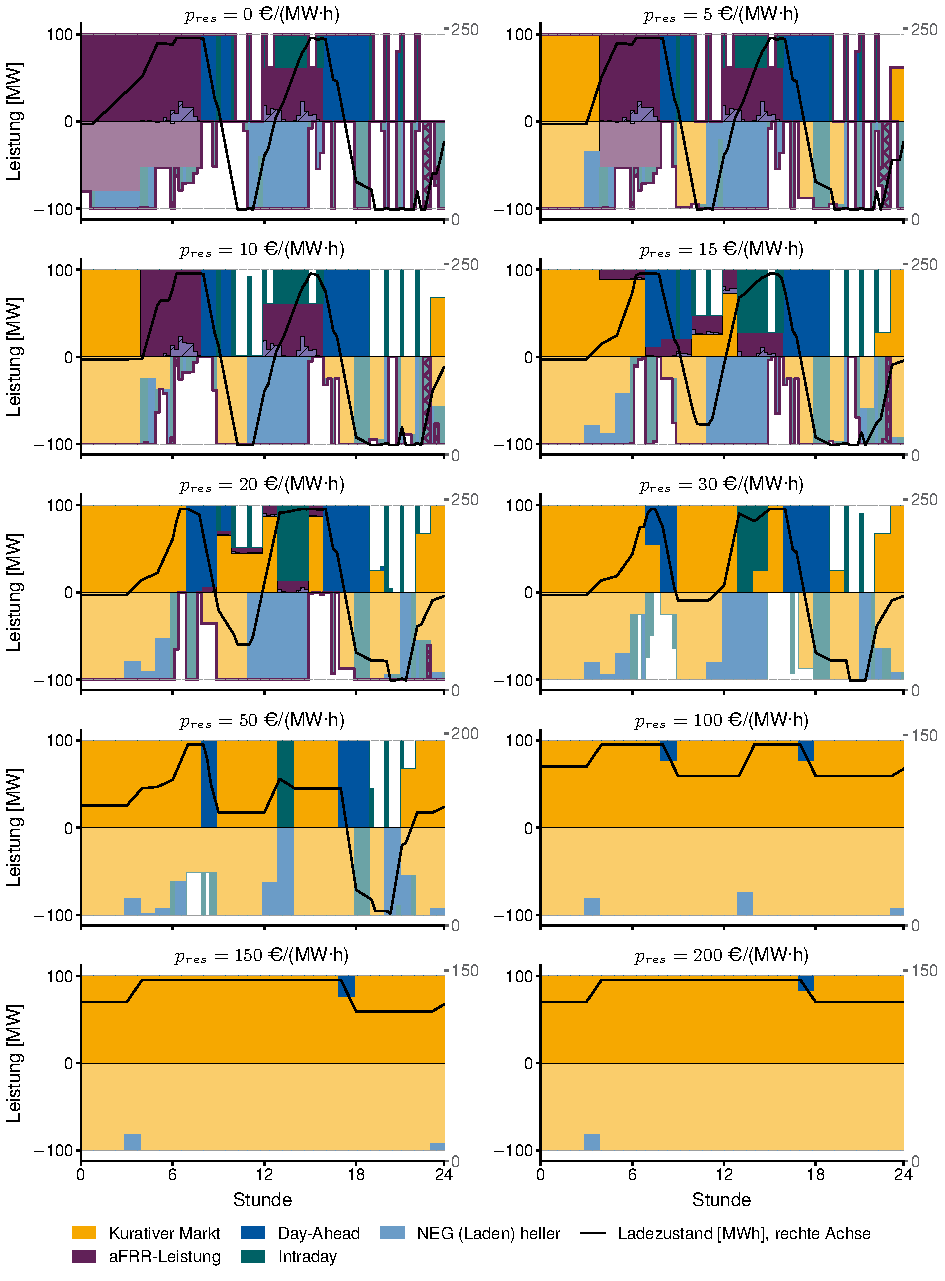
\includegraphics[width=\textwidth]{figures/anhang/dispatch_preisgitter_2025-01-20.pdf}
    \caption{Fahrplan und Ladezustand am 20.01.2025, dem Tag mit dem größten Spread am \acs{DA} des Jahres 2025, über zehn vorgegebene kurative Reservierungspreise von null bis 200\,\EurMWh{}.}
    \label{fig:preisgitter_2025_01_20}
\end{figure}

\begin{figure}[H]
    \centering
    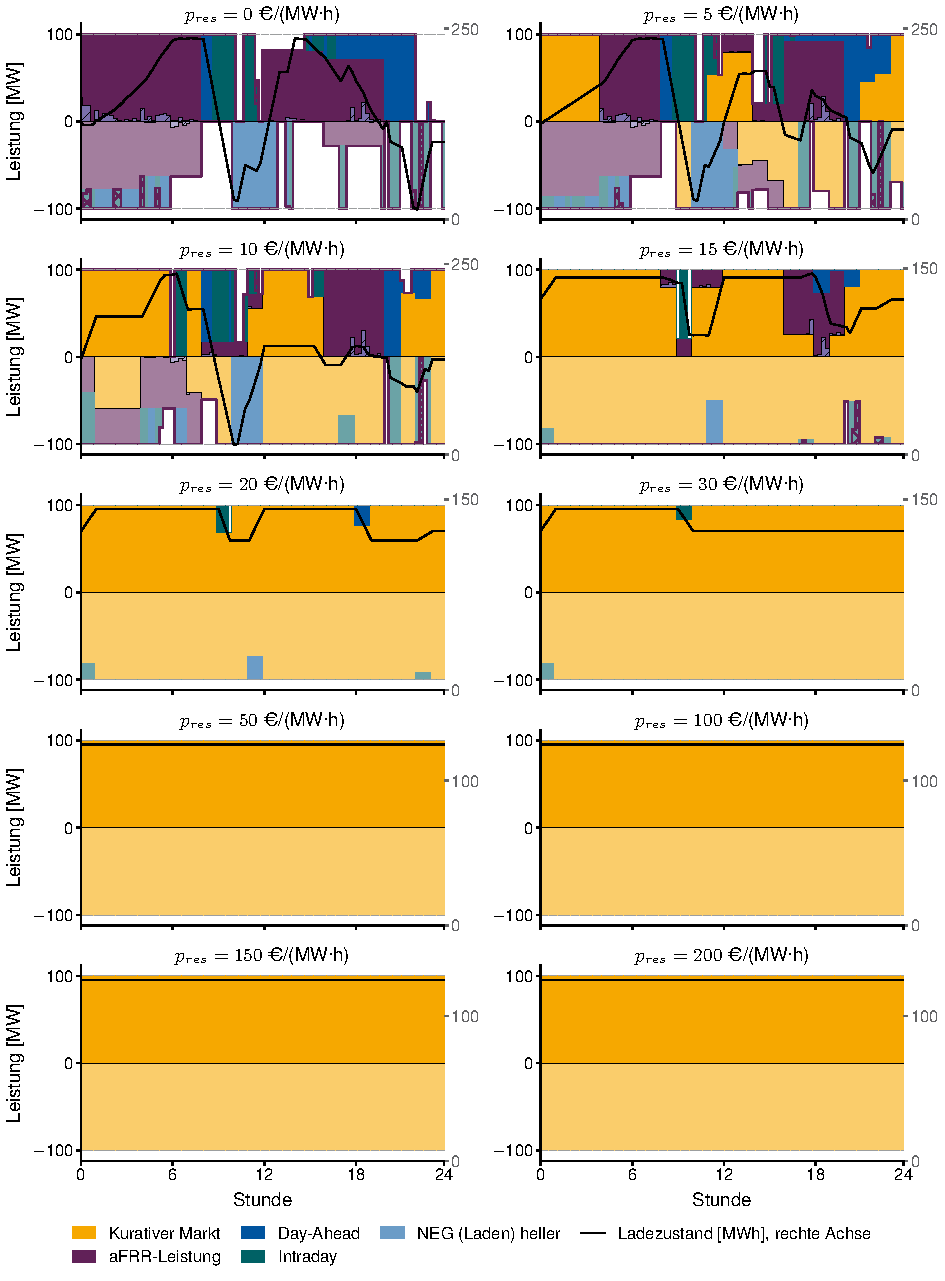
\includegraphics[width=\textwidth]{figures/anhang/dispatch_preisgitter_2025-02-11.pdf}
    \caption{Fahrplan und Ladezustand am 11.02.2025, dem Tag mit dem größten Redispatchbedarf des Jahres 2025, über zehn vorgegebene kurative Reservierungspreise von null bis 200\,\EurMWh{}.}
    \label{fig:preisgitter_2025_02_11}
\end{figure}

\begin{figure}[H]
    \centering
    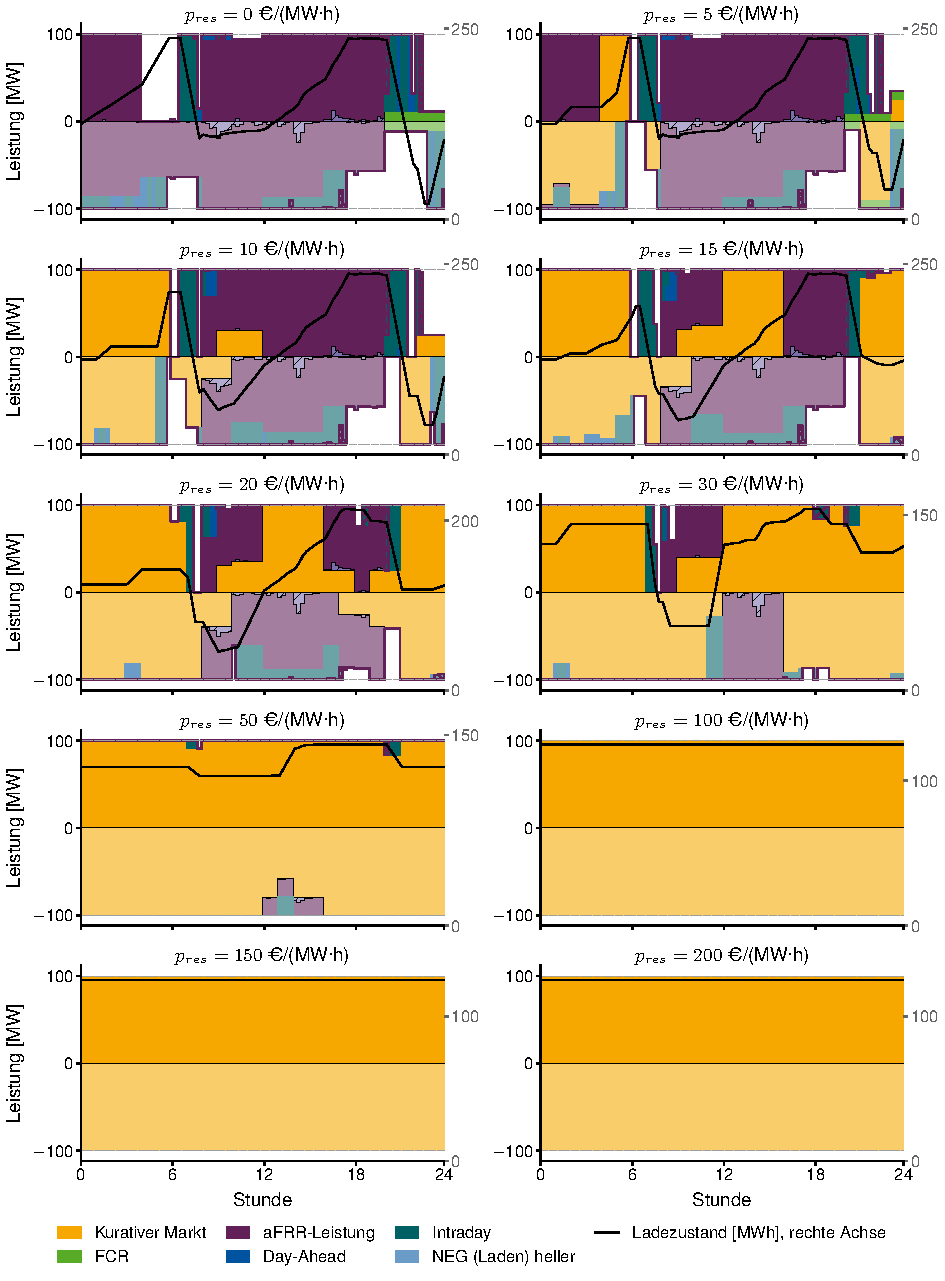
\includegraphics[width=\textwidth]{figures/anhang/dispatch_preisgitter_2025-05-06.pdf}
    \caption{Fahrplan und Ladezustand am 06.05.2025, einem Tag mit hohen Preisen der \acs{FCR} und niedrigen Preisen der \acs{aFRR}-Leistung, über zehn vorgegebene kurative Reservierungspreise von null bis 200\,\EurMWh{}.}
    \label{fig:preisgitter_2025_05_06}
\end{figure}

\begin{figure}[H]
    \centering
    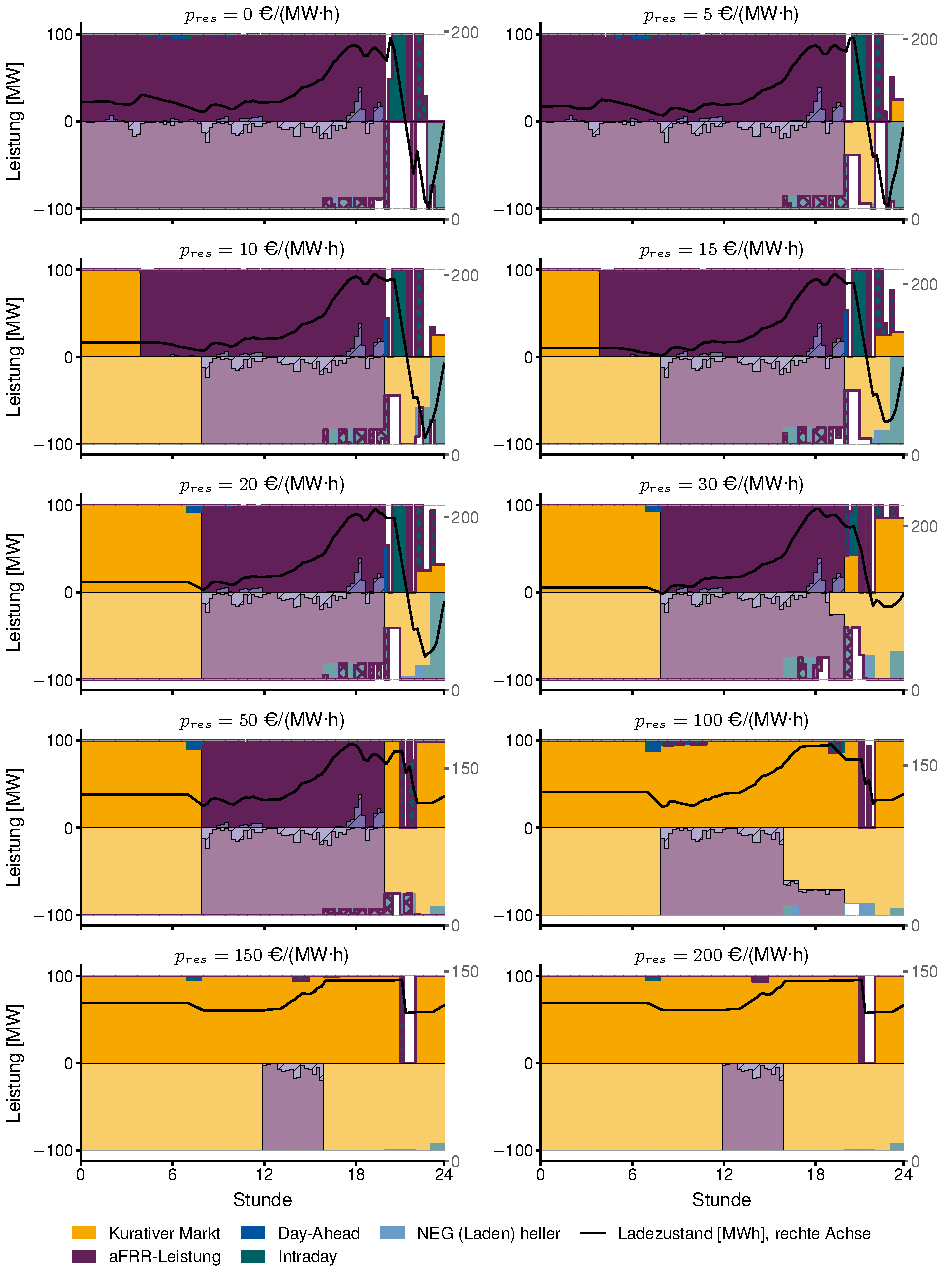
\includegraphics[width=\textwidth]{figures/anhang/dispatch_preisgitter_2025-05-15.pdf}
    \caption{Fahrplan und Ladezustand am 15.05.2025, dem Tag mit den höchsten Preisen der \acs{FCR} und der \acs{aFRR}-Leistung des Jahres 2025, über zehn vorgegebene kurative Reservierungspreise von null bis 200\,\EurMWh{}.}
    \label{fig:preisgitter_2025_05_15}
\end{figure}

\begin{figure}[H]
    \centering
    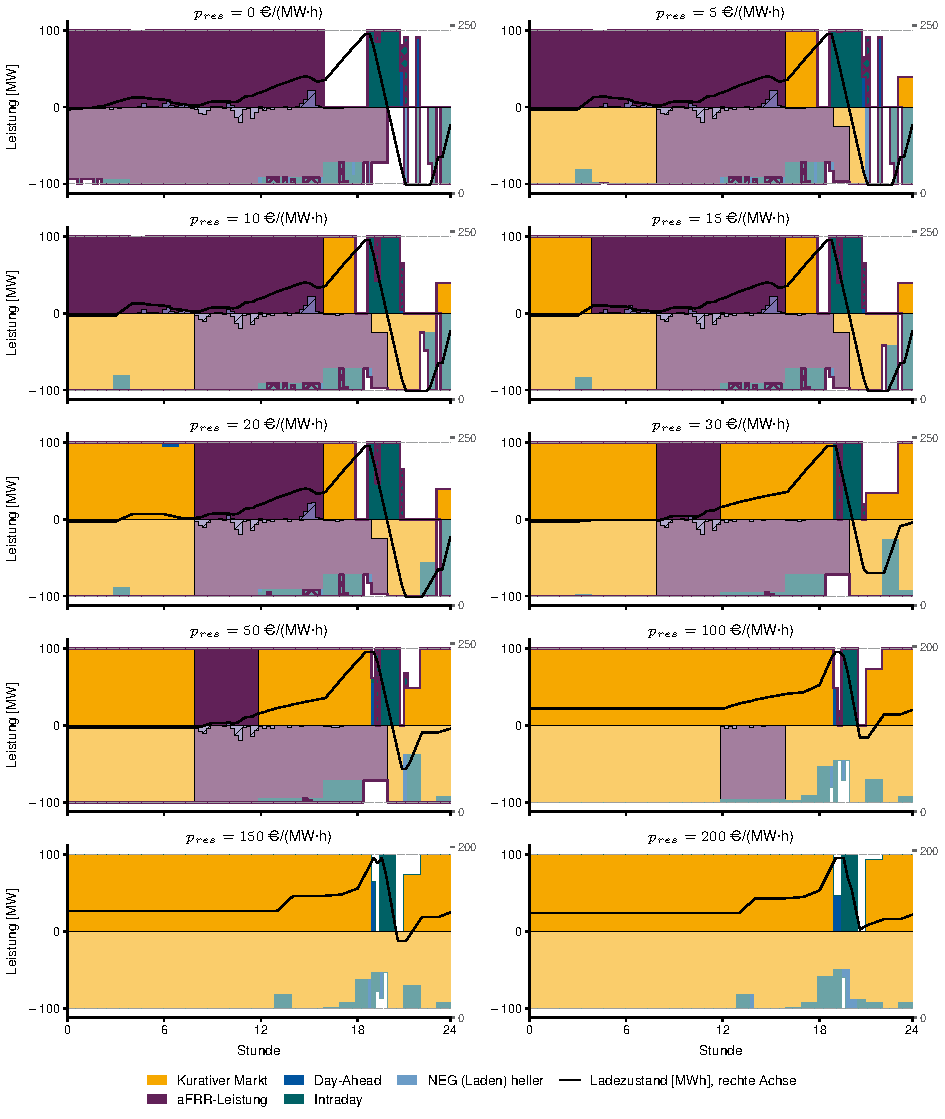
\includegraphics[width=\textwidth]{figures/anhang/dispatch_preisgitter_2025-08-26.pdf}
    \caption{Fahrplan und Ladezustand am 26.08.2025, dem Tag mit der größten Tagesspanne des \acs{ID1} des Jahres 2025, über zehn vorgegebene kurative Reservierungspreise von null bis 200\,\EurMWh{}.}
    \label{fig:preisgitter_2025_08_26}
\end{figure}
